\documentclass[]{article}
\usepackage{lmodern}
\usepackage{amssymb,amsmath}
\usepackage{ifxetex,ifluatex}
\usepackage{fixltx2e} % provides \textsubscript
\ifnum 0\ifxetex 1\fi\ifluatex 1\fi=0 % if pdftex
  \usepackage[T1]{fontenc}
  \usepackage[utf8]{inputenc}
\else % if luatex or xelatex
  \ifxetex
    \usepackage{mathspec}
  \else
    \usepackage{fontspec}
  \fi
  \defaultfontfeatures{Ligatures=TeX,Scale=MatchLowercase}
\fi
% use upquote if available, for straight quotes in verbatim environments
\IfFileExists{upquote.sty}{\usepackage{upquote}}{}
% use microtype if available
\IfFileExists{microtype.sty}{%
\usepackage{microtype}
\UseMicrotypeSet[protrusion]{basicmath} % disable protrusion for tt fonts
}{}
\usepackage[margin=1in]{geometry}
\usepackage{hyperref}
\hypersetup{unicode=true,
            pdftitle={Assignment 2},
            pdfauthor={Sri Seshadri},
            pdfborder={0 0 0},
            breaklinks=true}
\urlstyle{same}  % don't use monospace font for urls
\usepackage{graphicx,grffile}
\makeatletter
\def\maxwidth{\ifdim\Gin@nat@width>\linewidth\linewidth\else\Gin@nat@width\fi}
\def\maxheight{\ifdim\Gin@nat@height>\textheight\textheight\else\Gin@nat@height\fi}
\makeatother
% Scale images if necessary, so that they will not overflow the page
% margins by default, and it is still possible to overwrite the defaults
% using explicit options in \includegraphics[width, height, ...]{}
\setkeys{Gin}{width=\maxwidth,height=\maxheight,keepaspectratio}
\IfFileExists{parskip.sty}{%
\usepackage{parskip}
}{% else
\setlength{\parindent}{0pt}
\setlength{\parskip}{6pt plus 2pt minus 1pt}
}
\setlength{\emergencystretch}{3em}  % prevent overfull lines
\providecommand{\tightlist}{%
  \setlength{\itemsep}{0pt}\setlength{\parskip}{0pt}}
\setcounter{secnumdepth}{0}
% Redefines (sub)paragraphs to behave more like sections
\ifx\paragraph\undefined\else
\let\oldparagraph\paragraph
\renewcommand{\paragraph}[1]{\oldparagraph{#1}\mbox{}}
\fi
\ifx\subparagraph\undefined\else
\let\oldsubparagraph\subparagraph
\renewcommand{\subparagraph}[1]{\oldsubparagraph{#1}\mbox{}}
\fi

%%% Use protect on footnotes to avoid problems with footnotes in titles
\let\rmarkdownfootnote\footnote%
\def\footnote{\protect\rmarkdownfootnote}

%%% Change title format to be more compact
\usepackage{titling}

% Create subtitle command for use in maketitle
\newcommand{\subtitle}[1]{
  \posttitle{
    \begin{center}\large#1\end{center}
    }
}

\setlength{\droptitle}{-2em}
  \title{Assignment 2}
  \pretitle{\vspace{\droptitle}\centering\huge}
  \posttitle{\par}
  \author{Sri Seshadri}
  \preauthor{\centering\large\emph}
  \postauthor{\par}
  \predate{\centering\large\emph}
  \postdate{\par}
  \date{7/22/2018}


\begin{document}
\maketitle

\section{Problem 1}\label{problem-1}

\subsection{Model Formulation :}\label{model-formulation}

\subsubsection{Decision variables:}\label{decision-variables}

Let the number produced weekly for products A, B and C be
\(p_{a},p_{b}\) and \(p_{c}\)

\subsubsection{Objective function:}\label{objective-function}

\(Maximize\) \(Profit = Revenue - Cost\)

\(Revenue = 101p_{a} + 67p_{b} + 97.5p_{c}\)

\(Cost = (7*3p_{a} + 5*2p_{a} + 15*4_p{a}) + (7*p_{b} + 5*4p_{b} + 15*2p_{b}) + (7*5p_{c} + 15*3.5p_{c})\)

\subsubsection{Constraints:}\label{constraints}

\paragraph{Materials Used:}\label{materials-used}

Material 1 usage in lbs:

\(3p_{a} + p_{b} + 5p_{c} <= 300\)

Material 2 usage in lbs:

\(2p_{a} + 4p_{b} + 0p_{c} <= 400\)

\paragraph{Labor usage}\label{labor-usage}

Labor usage in hours:

\(4p_{a} + 2p_{b} + 3.5p_{c} <= 200\)

\paragraph{Weekly Demand and non negativity
constraint}\label{weekly-demand-and-non-negativity-constraint}

\(p_{a} >= 0, p_{b} >= 0 ,p_{c} >= 10\)

\subsection{ASPE Formulation and
results}\label{aspe-formulation-and-results}

Optimal Values are \(p_{a} = 0, p_{b} = 82 ,p_{c} = 10\)

\(Profit = 920\)

\begin{figure}
\centering
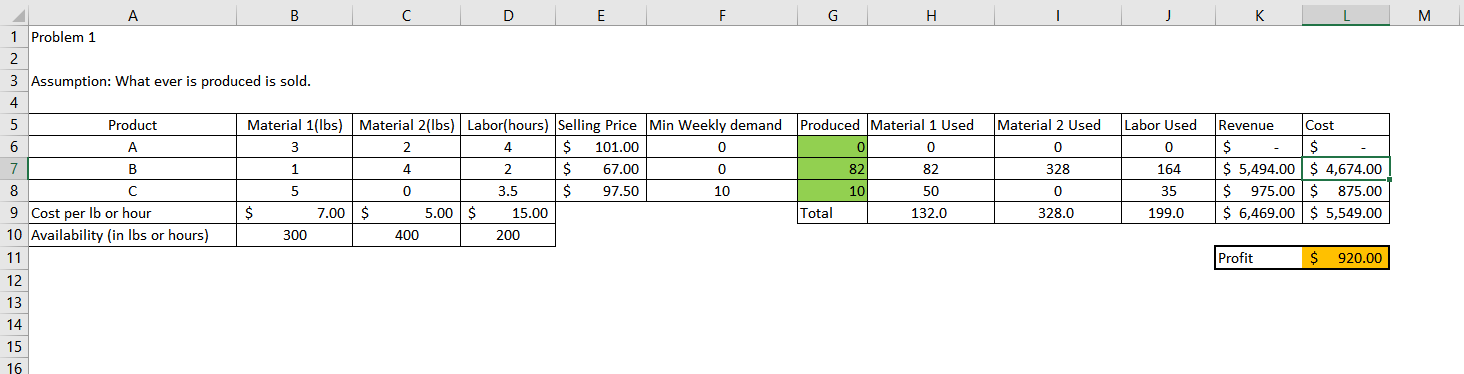
\includegraphics{Figures/Problem1.PNG}
\caption{Problem 1 ASPE formulation}
\end{figure}

\begin{figure}
\centering
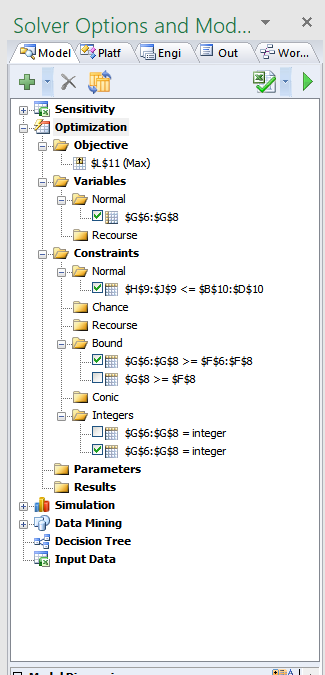
\includegraphics[height=0.50000\textwidth]{Figures/Problem1_Solver.PNG}
\caption{Problem 1 ASPE Model setup}
\end{figure}

\pagebreak

\section{Problem 2:}\label{problem-2}

\subsection{Model Formulation:}\label{model-formulation-1}

\subsubsection{Decision Variables:}\label{decision-variables-1}

Let \(F_{m},B_{m}\) be the number of footballs and baseballs produced in
the morning shift, likewise, \(F_{e},B_{e}\) be the number of footballs
and baseballs produced in the evening shift

\subsubsection{Objective function:}\label{objective-function-1}

\(Minimize\) \(Production\) \(Cost\) =
\(20F_{m} + 20B_{m} + 25F_{e} + 25B_{e}\)

\subsubsection{Constraints}\label{constraints-1}

\subsubsection{Labor Hours:}\label{labor-hours}

\(0.75F_{m} + 2B_{m} <= 5000\) \(0.75F_{e} + 2B_{e} <= 2000\)

\subsubsection{Leather used:}\label{leather-used}

\(7F_{m} + 15B_{m} <= 15000\) \(7F_{e} + 15B_{e} <= 14000\)

\subsubsection{Inner plastic usage:}\label{inner-plastic-usage}

\(0.5F_{m} + 2B_{m} <= 2000\) \(0.5F_{e} + 2B_{e} <= 1500\)

\subsubsection{Demand:}\label{demand}

\(F_{m} + F_{e} = 1500\) \(B_{m} + B_{e} = 1200\)

\subsubsection{Non negative constraint}\label{non-negative-constraint}

\(F_{m},B_{m},F_{e},B_{e} >= 0\)

\subsection{ASPE Formulation and
results:}\label{aspe-formulation-and-results-1}

\(F_{m} = 805,B_{m} = 624,F_{e} = 695,B_{e}= 576\)

\(Production\) \(Cost = 60355\)

\newpage

\begin{landscape}

![Problem 2 ASPE formulation](Figures\Problem2.PNG)

\end{landscape}

\begin{figure}
\centering
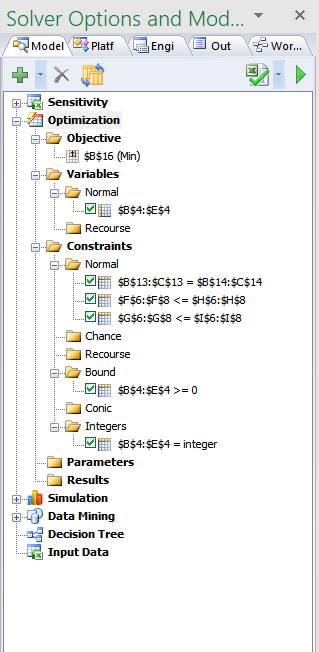
\includegraphics[height=0.70000\textwidth]{Figures/Problem2_Solver.PNG}
\caption{Problem 2 ASPE Model setup}
\end{figure}

\pagebreak

\section{Problem 3}\label{problem-3}

\subsection{Model formulation:}\label{model-formulation-2}

\subsubsection{Decision variables:}\label{decision-variables-2}

Let \(X_{i}\) be the number of firefighters starting their workday at
the begining of shift \(i\). \(i \in\ \{1,2,3,4,5,6\}\)

Where \(i\) in 1 through 6 are Midnight - 4am, 4 am - 8am, 8am - noon,
noon- 4pm, 4pm - 8pm and 8pm - Midnight

\subsubsection{Objective function}\label{objective-function-2}

\(Minimize\) \(\sum_{i=1}^{6}X_{i}\)

\subsubsection{Constraints}\label{constraints-2}

Number of firefighters in Shift 1:

\(X_{6} + X_{1} >= 5\)

Number of firefighters in Shift 2:

\(X_{1} + X_{2} >= 6\)

Number of firefighters in Shift 3:

\(X_{2} + X_{3} >= 10\)

Number of firefighters in Shift 4:

\(X_{3} + X_{4} >= 12\)

Number of firefighters in Shift 5:

\(X_{4} + X_{5} >= 8\)

Number of firefighters in Shift 6:

\(X_{5} + X_{6} >= 5\)

Non negative constraint

\(X_{i} >= 0\)

\subsection{ASPE Formulation and
results:}\label{aspe-formulation-and-results-2}

\(X_{1} = 5, X_{2} = 1, X_{3} = 9, X_{4} = 3, X_{5} = 5, X_{6} = 0\)

\(Total\) \(Firefighters = 23\)

\begin{figure}
\centering
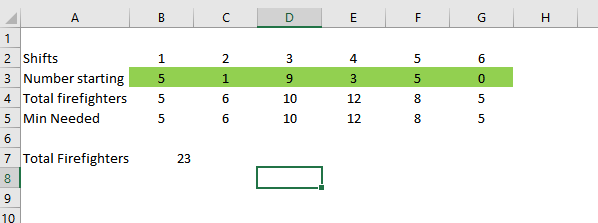
\includegraphics{Figures/Problem3.PNG}
\caption{Problem 3 ASPE formulation}
\end{figure}

\begin{figure}
\centering
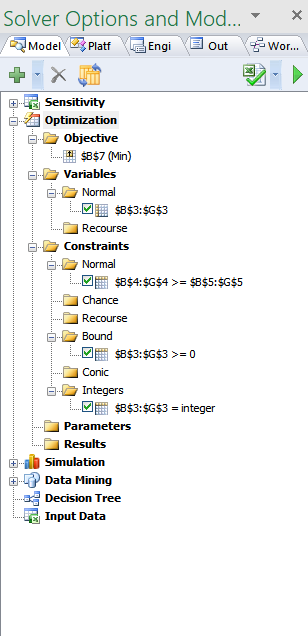
\includegraphics[height=0.50000\textwidth]{Figures/Problem3_Solver.PNG}
\caption{Problem 3 ASPE Model setup}
\end{figure}

\pagebreak

\section{Problem 4}\label{problem-4}

The problem statement can be interpreted multiple ways:

\begin{enumerate}
\def\labelenumi{\arabic{enumi}.}
\item
  The Labor cost is covered or sunk in the production cost and the
  maximum labor hours available for September through November is 1200
  and 1100 for December.
\item
  The labor cost is not sunk; 24 hours per day is available as labor
  hours per product and management pays only 1000 hours of labor for
  upto 1200 hours for Sep - Nov and pays the variable cost of labor for
  anything exceeding 1200 hours for Sep - Nov. (likewise for Dec,
  management pays for 1000 hours for upto 1100 hours and pays the hourly
  rate for hours beyond 1100.)
\item
  The holding cost could be calculated on the average inventory for the
  month OR on the ending inventory per month. In this problem the
  holding cost is calculated for the average invetory for the month.
\end{enumerate}

\subsection{Scenario 1 - Assuming labor cost is sunk in production
cost.}\label{scenario-1---assuming-labor-cost-is-sunk-in-production-cost.}

\subsubsection{Decision Variables:}\label{decision-variables-3}

Let \(S_{i}\) and \(H_{i}\) be the number of standard and heavy pumps
produced in month \(i\). Where \(i \in \{9,10,11,12\}\)

\subsubsection{Objective function}\label{objective-function-3}

\(Minimize\) \(Total Cost = Production Cost + Holding Cost\)

Let \(Ps_{i}\) and \(Ph_{i}\) be the production cost for standard and
heavy duty pumps for the months i.

\(Production Cost = \sum_{i=9}^{12}(S_{i}*Ps_{i} + H_{i}*Ph_{i})\)

Let \(Ds_{i}\) and \(Dh_{i}\) be the demand for standard and heavy duty
pumps for the months i. Let \(Bs_{i}\) and \(Bh_{i}\) be the beginning
inventory for standard and heavy duty pumps for the months i. Let
\(Es_{i}\) and \(Eh_{i}\) be the ending inventory for standard and heavy
duty pumps for the months i.

Where \(Bs_{9} = Bh_{9} = 0\) and
\(Bs_{i+1} = Es_{i} ; Bh_{i+1} = Eh_{i}\)
\(Es_{i} = Bs_{i} + Ps_{i} - Ds_{i} ; Eh_{i} = Bh_{i} + Ph_{i} - Dh_{i}\)

\(Holding Cost = (\sum_{i=9}^{12}\frac {1}{2}*5(Bs_{i} + Bh_{i} + Es_{i} + Eh_{i}))\)

\subsubsection{Constraints}\label{constraints-3}

\paragraph{Ending inventory:}\label{ending-inventory}

\(\sum_{i=9}^{i=12}(Es_{i} + Eh_{i}) <= 1800\) \(Es_{12} >= 800\)
\(Fh_{12} >= 850\)

\paragraph{Monthly labor hours:}\label{monthly-labor-hours}

\(0.45Ps_{i} + 0.52Ph_{i} >= 1000\) \(i \in \{9,10,11,12\}\)

\(0.45Ps_{i} + 0.52Ph_{i} <= 1200\) \(i \in \{9,10,11\}\)

\(0.45Ps_{12} + 0.52Ph_{12} >= 1100\)

\subsubsection{Non negative constraints}\label{non-negative-constraints}

\(Ps_{i} >= 0\) and \(Ph_{i} >= 0\)

\subsubsection{ASME formulation \&
results}\label{asme-formulation-results}

\(Ps_{9} = 650, Ps_{10} = 875, Ps_{11} = 790, Ps_{12} = 1900\)
\(Ph_{9} = 1745, Ph_{10} = 1265, Ph_{11} = 1240, Ph_{12} = 350\)

\(Total Cost = 1,260,196.59\)

\begin{figure}
\centering
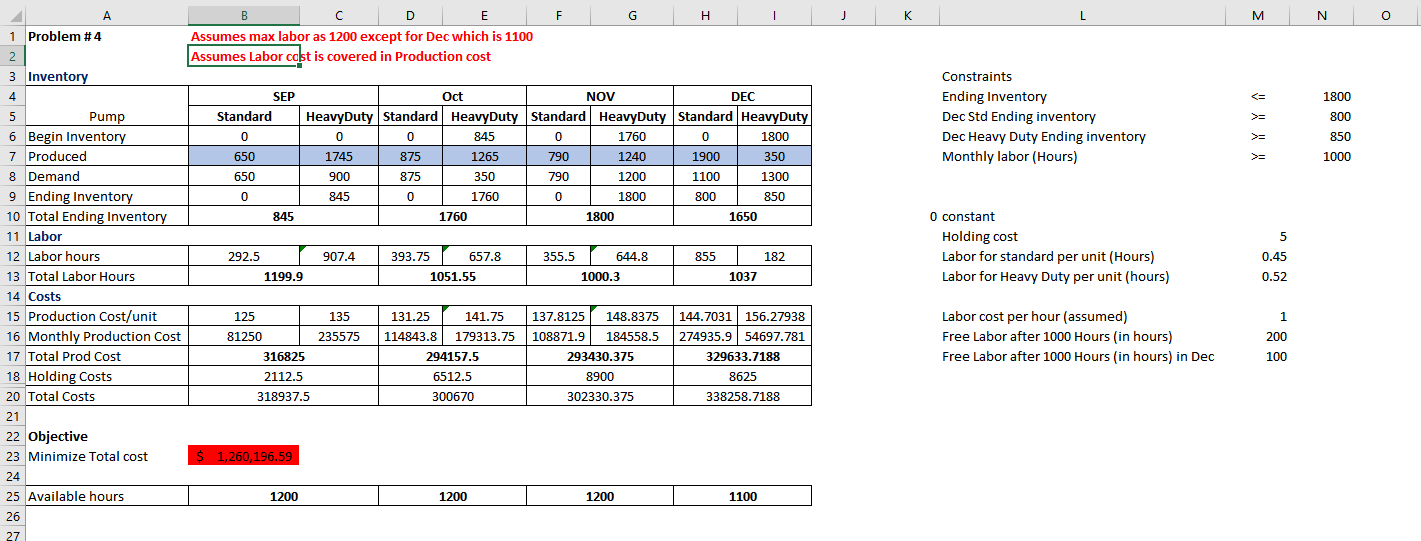
\includegraphics{Figures/Problem4S1.PNG}
\caption{Problem 4 Scenario 1 ASPE formulation}
\end{figure}

\begin{figure}
\centering
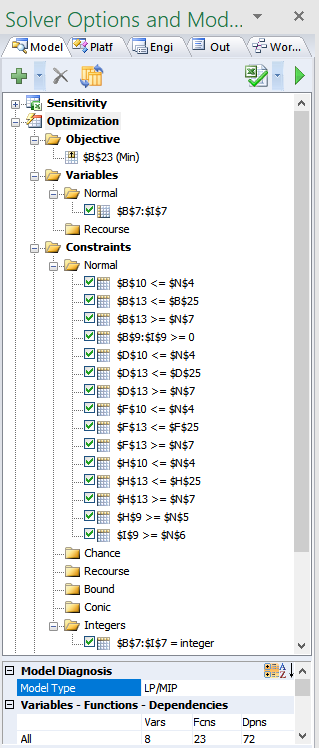
\includegraphics[height=0.30000\textwidth]{Figures/Problem4S1_Solver.PNG}
\caption{Problem 4 Scenario 1 ASPE Model setup}
\end{figure}

\pagebreak

\subsection{Scenario 2 - Assuming labor cost is NOT sunk in production
cost. And there is access to labor hours of 1440 for Sep and Nov and
1448 hours for Oct and
Dec.}\label{scenario-2---assuming-labor-cost-is-not-sunk-in-production-cost.-and-there-is-access-to-labor-hours-of-1440-for-sep-and-nov-and-1448-hours-for-oct-and-dec.}

Here we add labor cost assuming \$1 per hour of labor, any labor rate
can be assumed, the optimal values do not change.

if \(0.45Ps_{i} + 0.52Ph_{i} >= 1200\) then labor cost
\(= 1000 + 1200 - (0.45Ps_{i} + 0.52Ph_{i})\) else labor cost = 1000 for
\(i \in \{9,10,11\}\)

if \(0.45Ps_{12} + 0.52Ph_{12} >= 1100\) then labor cost
\(= 1000 + 1100 - (0.45Ps_{12} + 0.52Ph_{12})\) else labor cost
\(= 1000\)

The objective function would now include the labor cost as well

\(Minimize\)
\(Total Cost = Production Cost + Holding Cost + Labor Cost\)

Labor constraints would be modified as

\(0.45Ps_{i} + 0.52Ph_{i} >= 1000\) \(i \in \{9,10,11,12\}\)

\(0.45Ps_{i} + 0.52Ph_{i} <= 1440\) \(i \in \{9,11\}\)

\(0.45Ps_{i} + 0.52Ph_{i} <= 1488\) \(i \in \{10,12\}\)

\subsubsection{ASME formulation \&
results}\label{asme-formulation-results-1}

\(Ps_{9} = 650, Ps_{10} = 875, Ps_{11} = 790, Ps_{12} = 1900\)
\(Ph_{9} = 1844, Ph_{10} = 1166, Ph_{11} = 1240, Ph_{12} = 350\)

\(Total Cost = 1,260,074.72\)

\begin{figure}
\centering
\includegraphics[height=1.50000\textwidth]{Figures/Problem4S2.PNG}
\caption{Problem 4 Scenario 2 ASPE formulation}
\end{figure}

\begin{figure}
\centering
\includegraphics[height=0.40000\textwidth]{Figures/Problem4S2_Solver.PNG}
\caption{Problem 4 Scenatio 2ASPE Model setup}
\end{figure}

\pagebreak

\section{Problem 5}\label{problem-5}

\begin{enumerate}
\def\labelenumi{\alph{enumi})}
\item
  Small offices = 3, Large offices = 44
\item
  Optimal monthly revenue = 48,050
\item
  remaining or unused square footage = 51,800
\item
  Since the increase is within the allowable increase, the optimal
  values do not change. The objective function value would change to
  \$48,650
\item
  The Shadow price is 0 for the square footage and the constraint on
  square footage is non-binding, hence increase in square footage does
  not impact the objective function.
\item
  The ratio of increase to allowable increase (50/400) and the ratio of
  decrease to allowable decrease (200/250) sum up to \textless{} 1,
  there is no impact in the optimal values. The objective function
  changes to \$39,400.
\end{enumerate}

\section{Extra Credit}\label{extra-credit}

\(X_{1} + X_{2} + X_{3} <= 5\)

\(-X_{1} + X_{2} + 2X_{3} <= 6\)

\(X_{1},X_{2},X_{3} >= 0\)

There are 3 variables and 2 inequality equations. We'll use the Simplex
method to identify Optimal solution for \(Max \sum_{i=1}^{3}X_{i}\).

We'll add 2 slack variables to create equality in the above inequalities

\(X_{1} + X_{2} + X_{3} + S_{1} = 5\)

\(-X_{1} + X_{2} + 2X_{3}+ S_{2} = 6\)

The following table shows the Corner points in blue.

\begin{figure}
\centering
\includegraphics[height=1.50000\textwidth]{Figures/ExtraCreditSimplex.PNG}
\caption{Problem 5}
\end{figure}


\end{document}
